\chapter{Introduction}

\textbf{Author: Lukas Leskovar}

\vspace{2mm}

\section{The Evolution of Robotics}


Robotic research has always utilized concepts, processes, and methods of different scientific disciplines such as physics, mathematics, and biology to improve application and aid human needs. Because of this industrial, medical and even agricultural sectors have used technologies and products developed by researchers to improve workflows and alleviate employees from performing exhausting tasks. This relationship ranges back to the early ages of information technology in the 1950s and 1960s in which many developments on production robots and Artificial Intelligence (AI) have been made.
Between 1970 and 1990 the public interest in automation and AI has decreased forcing the industry into the so-called AI winter. Despite this recession, research has been continued and the building blocks for another robot boom during the 1990s have been set. Since then the usage of robotic applications has broadened and the industry has proven itself to be a vital aspect of today's economy.

\begin{figure}
	\centering
	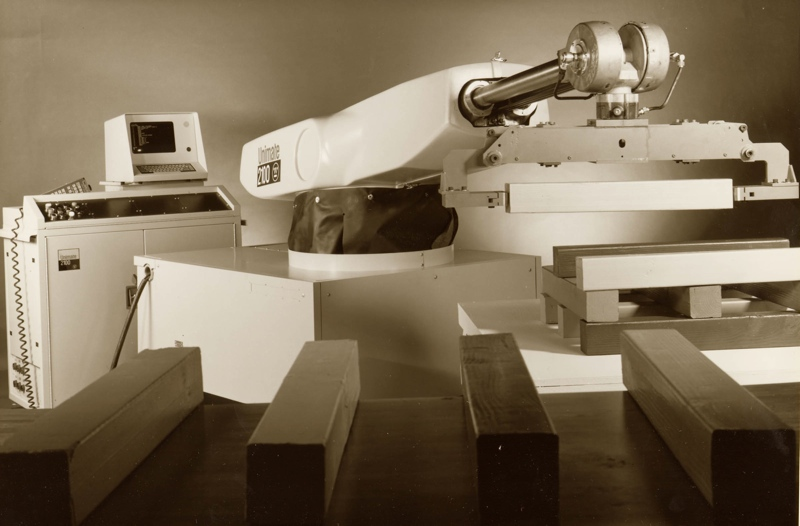
\includegraphics[width=0.7\linewidth]{img/unimate}
	\caption{
		Picture of the first industrial robot. The Unimate developed by George Devol and Joseph Engelbert in 1961 was first used for hot die-casting and welding applications.\protect\footnotemark[1]
	}
	\label{fig:unimate}
\end{figure}
\addtocounter{footnote}{+1}\footnotetext{\cite{malone2011unimate}}

\section{Robots with human interaction}
Nowadays the utilization of robots in workplaces has broadened to almost every branch and is accepted by employees and workers. In countries like Japan, robots are no longer seen as a threat to jobs. 
%noch ein sanfterer Übergang 
Industrial robots are no longer used as simple construction tools, their safety and accuracy have improved so that collaborative robots (Cobots) are capable of working in close cooperation with humans. 
Surgery robots used in the medical sector not only allow for much more accurate procedures but also enable remote specialists to work on patients without having to be in the same hospital. 
In developed countries, educational robots are used at school or at home to teach children topics in a playful and interesting way.

\section{Robots in hazardous environments}
Robots do not only serve a purpose in a close-to-user work environment, they also ensure human safety by performing dangerous tasks in unsafe surroundings. 
Remotely controlled robots or drones can be used for inspecting mine shafts, collapsed buildings, pipelines, or overhead power poles.
Other applications of such robots are bomb or mine defusion, fire extinction, or avalanche rescue.

\section{Autonomous robots}
Implementing an autonomous robot system is an intricate task that proposes many challenging problems for research or development teams. Autonomy requires a system to continuously work in a dynamic environment without external controlling inputs and utilize perceived information about its surroundings to adapt to environmental change. \footcite[Pages 1-2]{bekey2005autonomous}
Despite their complexity in development autonomous systems, mobile or stationary, immensely facilitate the execution of a job for the human user.
Such robots can be used to navigate and organize warehouses, constructing parts in an assembly line, or map large areas for comprehensive calculations.

\section{3D Mapping}
%eigentlich möche ich noch den 3D Mapping Markt erwähnen


\section{Autonomous 3D Mapping}
While 3D Mapping is a well-established and growing economy most applications require human interaction at some point during the mapping process. Products such as the Emesent Hovermap \footcite{hovermap2021} or Exyn Aero \footcite{exynAero2021} utilize the spatial flexibility of drones and high-end light detection and ranging (LiDAR) Sensors to facilitate autonomous mapping in GPS-denied areas without being within sight of the drone pilot. These solutions are used to autonomously map building or explore hazardous environments such as mineshafts in a human-safe manner as seen in Fig. \ref{fig:hovermap}.

\begin{figure}
	\centering
	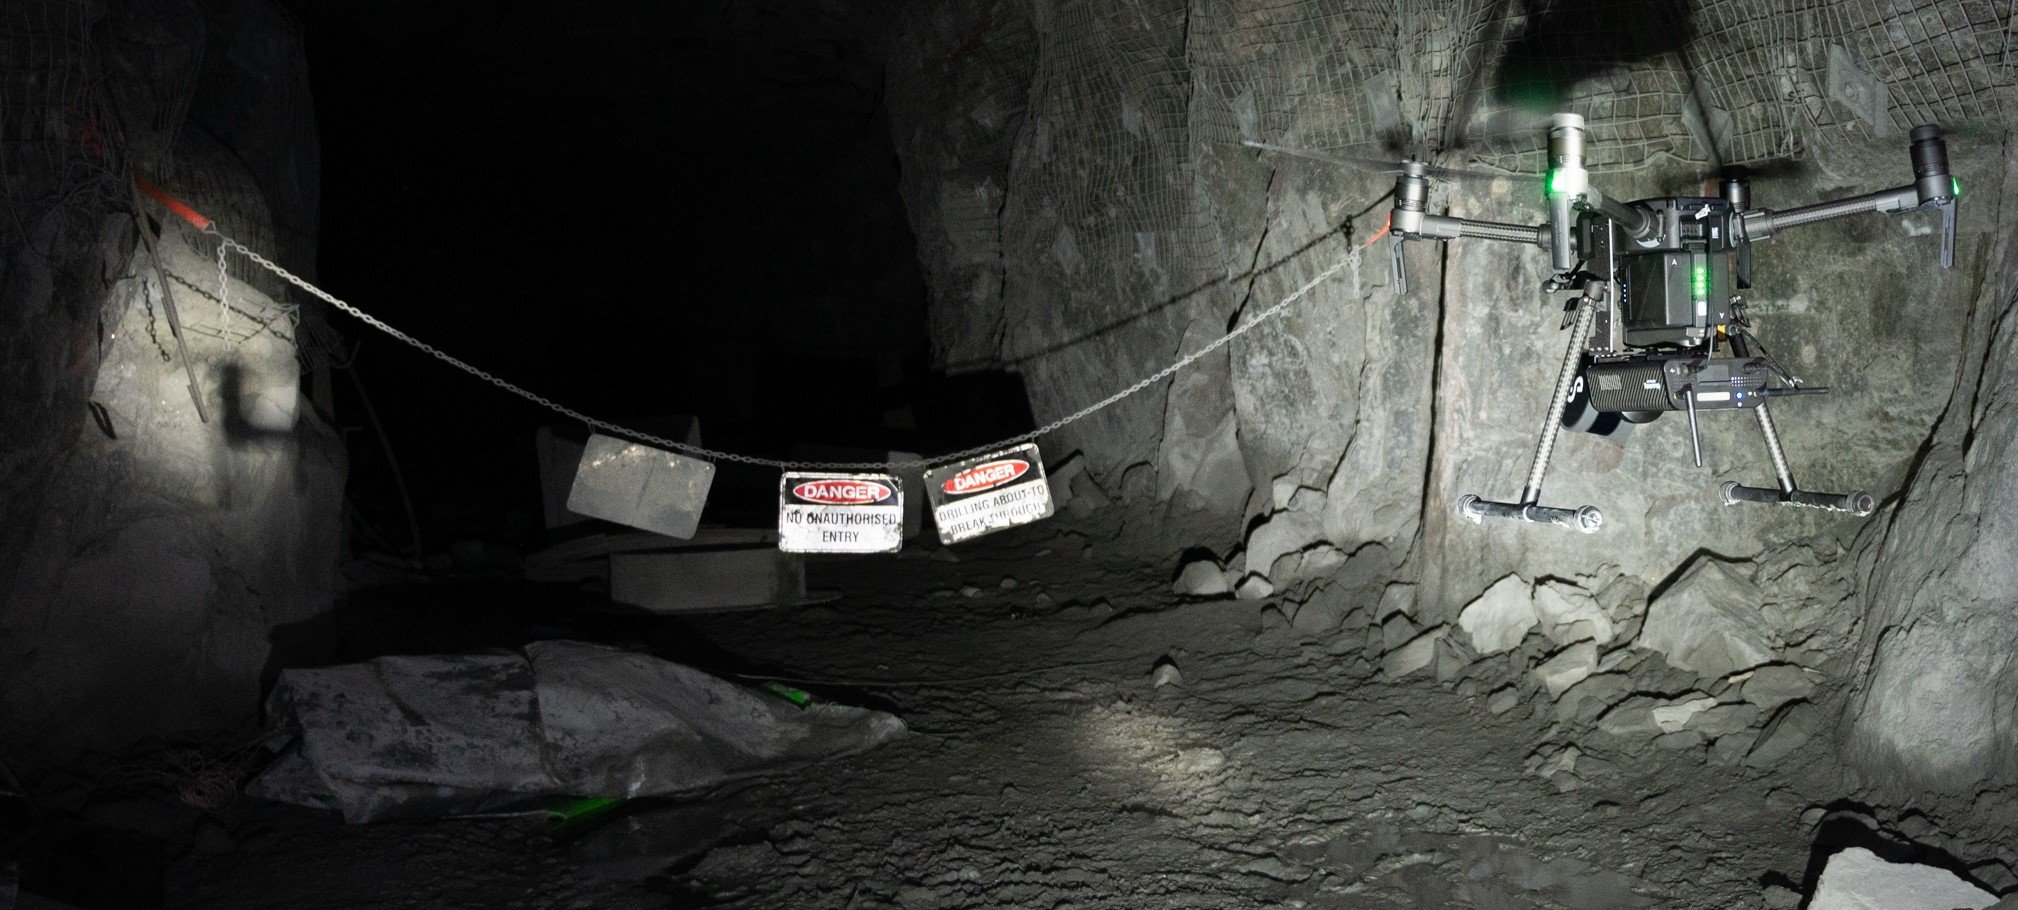
\includegraphics[width=0.9\linewidth]{img/hovermap}
	\caption{
		The Emesent Hovermap mapping a dangerous area inside a mineshaft.\protect\footnotemark
	}
	\label{fig:hovermap}
\end{figure}
\footnotetext{\cite{hovermapIMG}}

\section{Goals}
The project associated with this thesis aims to implement a 3D Mapping system similar to the aforementioned solutions with limited financial, personnel as well as temporal resources. This goal forces the project team to primarily maintain an open-source approach during development.

The goal of this thesis is to document the challenges encountered and experiences gained by the project team during development to demonstrate how highly sophisticated industrial problems can be solved in a low-budget fashion. 
%noch bisschen mit "wir machen das für jüngerere Schüler" flexen, etc...


\section{Requirements}
%noch besser formulieren nicht nur abschreiben vom Projektantrag
In order to declare the project as successful the following criteria have to be implemented:
\begin{itemize}
	\item The system is capable of generating a 3D Point-cloud of its surroundings
	\item All required hardware (e.g. sensors, computing boards, etc.) is mounted onto a drone-platform 
	\item All calculations concerning the map-generation are run on a external server in direct communication with the drone
	\item The drone utilizes the Point-cloud to orientate in its surroundings and navigate one ore multiple waypoints
	\item The drone is capable of avoiding obstacles as it is moving through a unknown environment
\end{itemize}

The following criteria can be implemented but have no direct correlation to the success of the project:
\begin{itemize}
	\item A Web-App facilitating the usage of the system and enabling the user to create waypoints, monitor the drone and mapping algorithm as well as evaluate the Point-cloud
	\item The system is replicated within the gazebo simulator to simplify future development without direct access to its hardware
\end{itemize}


\filbreak
